
%(BEGIN_QUESTION)
% Copyright 2003, Tony R. Kuphaldt, released under the Creative Commons Attribution License (v 1.0)
% This means you may do almost anything with this work of mine, so long as you give me proper credit

Qualitatively determine the voltages across all components as well as the current through all components in this simple RC circuit at three different times: (1) just before the switch closes, (2) at the instant the switch contacts touch, and (3) after the switch has been closed for a long time.  Assume that the capacitor begins in a completely discharged state:

$$\includegraphics[width=15.5cm]{i00598x01.eps}$$

Express your answers qualitatively: ``maximum,'' ``minimum,'' or perhaps ``zero'' if you know that to be the case.

\vskip 10pt
\goodbreak

\noindent
{\bf Before the switch closes:}

$V_{C}$ = 

$V_{R}$ = 

$V_{switch}$ = 

$I$ = 

\vskip 10pt
\goodbreak

\noindent
{\bf At the instant of switch closure:}

$V_{C}$ = 

$V_{R}$ = 

$V_{switch}$ = 

$I$ = 

\vskip 10pt
\goodbreak

\noindent
{\bf Long after the switch has closed:}

$V_{C}$ = 

$V_{R}$ = 

$V_{switch}$ = 

$I$ = 

\vskip 10pt

Hint: a graph may be a helpful tool for determining the answers!

\vskip 20pt \vbox{\hrule \hbox{\strut \vrule{} {\bf Suggestions for Socratic discussion} \vrule} \hrule}

\begin{itemize}
\item{} A detail many students of electronics struggle to remember is whether or not capacitors oppose changes in {\it voltage} or changes in {\it current}.  One way to better remember this important fact is to link it to fundamental principles of physics you already know well such as the {\it Conservation of Energy}.  Explain whether {\it voltage} or {\it current} is the conserved quantity for a capacitor following a sudden circuit change based on what you know about how capacitors store energy.
\item{} In this ``experiment,'' is the capacitor {\it absorbing} energy or {\it releasing} energy?
\item{} Explain what will happen in the circuit when the switch is re-opened after the switch has been closed for a long period of time.
\end{itemize}

\underbar{file i00598}
%(END_QUESTION)





%(BEGIN_ANSWER)

\noindent
{\bf Before the switch closes:}

$V_{C}$ = zero

$V_{R}$ = zero

$V_{switch}$ = maximum

$I$ = zero

\vskip 10pt
\goodbreak

\noindent
{\bf At the instant of switch closure:}

$V_{C}$ = zero

$V_{R}$ = maximum

$V_{switch}$ = zero

$I$ = maximum

\vskip 10pt
\goodbreak

\noindent
{\bf Long after the switch has closed:}

$V_{C}$ = maximum

$V_{R}$ = zero

$V_{switch}$ = zero

$I$ = zero

\vskip 10pt

Follow-up question: which of these variables remained the same immediately before and immediately after switch closure?  Explain why.

%(END_ANSWER)





%(BEGIN_NOTES)

The purpose of this question is to preview the concept of ``initial'' and ``final'' values in RC circuits, before they learn to use the ``universal time constant formula.''

%INDEX% Electronics review: RC circuit ``initial'' and ``final'' values

%(END_NOTES)


